\chapter{Modeling Attempts}

\section{Simple ODE model (First Iteration)}
Here, we develop a model that keeps track of the following variables
\begin{quote}
	$n(t)$= density of tip cells in area of interest, (number per unit area).
	
	$\rho(t)$ = density of blood vessels (length per unit area).
	
	$c(t)$ = concentration of drug delivered to region by blood vessels (nano mole per unit area).
\end{quote}
An updating list of model parameters:
\begin{itemize}
	\item $v$ [length/time]: The rate at which the tip cells move and extends the blood vessels.
	\item $\delta_v$ [1/time]: The rate at which the vascular structure gets degraded.
	\item $\lambda_s$ [1/time]: Tip cell division rate (splitting rate).
	\item $\lambda_b$ [1/time/length]: Tip cell emerging rate from stalk cells.
	\item $\delta_t$ [1/time]: Tip cell death/deactivation rate.
	\item $\kappa$ [area/length/time]: Re-connection of tip cells to the other capillaries to form loops.  
	\item $\mu$ [1/time]: Permeability of the capillary to the drug. 
	\item $\sigma$ [area/length]: The coverage of the blood vessels in the region.
\end{itemize}
And a list input functions
\begin{itemize}
	\item $f(t)$: [nmol/length]: The amount of drug inside the capillary.
\end{itemize}




\subsection*{Studying dynamics of vessel formation}
\[ \frac{d\rho}{dt} = ??. \]
The active tip cells extend the vascular structure as they move. Assuming the tip cells move at rate $v$, then 
\[ \frac{d \rho}{dt} = vn+ ??. \]
Also, assuming the vascular structure degrades with rate $\delta$ [per unit time], we can add the degradation term 
\[ \boxed{\frac{d\rho}{dt} = vn - \delta_v \rho} . \]



\subsubsection*{Studying the Dynamics of Tip Cells}
Things important in the dynamics of the tip cells
\begin{itemize}
	\item Generation of the tip cells: There are at least two ways for new tip cell generation listed as follows:
	\begin{enumerate}[(i)]
		\item Splitting mechanics: When the tip cells splits new vascular stem gets two heads. This should be proportional to the density of tip cells. The parameter $\lambda_s$ [per unit time] reflects this mechanism.
		\item Branching: New tip cells can form out the the endothelial stalk cells. This process should be proportional to the density of blood vessels. The parameter $\lambda_b$ [per unit time per unit length] reflects this mechanism
	\end{enumerate}
	\item Loss of tip cells
	\begin{enumerate}[(i)]
		\item Death of the tip cells or getting deactivated: Reflected by the parameter $\delta_t$
		\item Joining the other branches of vascular network: When a tip cell reconnects another capillary branch, then they disappear. The parameter $\kappa$ is for this mechanism. Note that the re-connection term is proportional to both number of tips cells, as well as the density of blood vessels. Thus the units of $\kappa$ should be [area/length/time]. 
	\end{enumerate}
	\item The movement of tip cells and formation of new vascular networks along the way.
\end{itemize}

\[ \boxed{\frac{dn}{dt} = (\lambda_s - \delta_t) n + \lambda_b \rho - \kappa n \rho}.  \]

\subsubsection*{Nondimensionalization}
In order the analyze the model more easily, we nondimensionalize the system with the following change of variable
\[ \rho = R \tilde{\rho}, \qquad n = N \tilde{n}, \qquad t = T \tau. \]
There are many possible choice to choose the scaling factors $R, N, T$. However, we will choose them in a way that they are always positive, and the system of ODE becomes as simple as possible. Substituting the change of variable above in the ODE system, we will get
\begin{align*}
	&\frac{d\tilde{\rho}}{d\tau} = \frac{vNT}{R}\tilde{n} - \delta_v T \tilde{\rho},\\
	&\frac{d\tilde{n}}{d\tau} = T(\lambda_s-\delta_t)\tilde{n} + \frac{\lambda_b T R}{N} \tilde{\rho} - T\kappa R \tilde{n}\tilde{\rho}. \tag{\twonotes}
\end{align*}
We choose the following values for $T,N$, and $R$
\[ T = \frac{1}{\delta_v}, \qquad R = \frac{\delta_v}{\kappa}, \qquad N = \frac{\lambda_b}{\kappa}. \]
This is a very suitable moment to pause and check the dimensions if they match (I did it and all of them matches!). With these choices from the coefficients, the system of ODEs will be
\[ \frac{d\tilde{n}}{d \tau} = \frac{\lambda_s - \delta_t}{\delta_v} \tilde{n} + \tilde{\rho} - \tilde{n}\tilde{\rho}, \qquad
\frac{d\tilde{\rho}}{d\tau} = \frac{v\lambda_b}{\delta_v^2}\tilde{n} - \tilde{\rho}. \]
To make the ODEs simpler to work with, we will write $n,\rho$ in place of $\tilde{n}$ and $\tilde{\rho}$, and also we introduce the following parameters
\[ \alpha = \lambda_s - \delta_t, \qquad \beta =\delta_v, \qquad \gamma = v\lambda_b. \tag{$\clubsuit$} \]
Then we can write
\begin{equation*}
	\boxed{
		\begin{aligned}
			&\dot{n} = \frac{\alpha}{\beta}n + \rho - n\rho, \\
			&\dot{\rho} = \frac{\gamma}{\beta^2}n -\rho.
		\end{aligned}
	}
	\tag{\smiley}
\end{equation*}
In order to find the equilibrium points, we demand $\dot{n} = 0$ as well as $\dot{\rho} = 0$. This will lead to the following equations
\begin{align*}
	\dot{n} = 0&: \qquad \frac{\alpha}{\beta} n + \rho - n\rho = 0, \\
	\dot{\rho} =0&: \qquad \frac{\gamma}{\beta^2}n - \rho = 0.
\end{align*}
After some algebra, it turns out that there are two equilibrium points for this system.
\[ p^0_1 = (0,0), \qquad p^0_2 = (\frac{\alpha\beta}{\gamma} + 1, \frac{\gamma}{\beta^2}+\frac{\alpha}{\beta}) = (\frac{\alpha\beta+\gamma}{\gamma},\frac{\gamma + \alpha\beta}{\beta^2}). \tag{E.1.1} \]
%\begin{strangeObs}
%	Something does not make sense! We know that the variables $n$ and $\rho$ must all be positive, as they are both representing biological values. However, by looking closely at the second component of $p^0_2$, it turns out th at $\gamma - \alpha\beta$ should be positive. In order to have the first component positive as well, then $\gamma$ should be negative, which is not possible. That is because by $(\clubsuit)$ we know that $\gamma>0$. There is at least one solution for this paradox, which is letting $\alpha\beta - \gamma =0$. Then this equilibrium point will be the same as $p^0_1$, showing the fact that the system has only one equilibrium point with biological meaning, which is the origin (not very interesting)!\\
%	However, I am going to ignore this observation for now and proceed with the stability analysis.
%	
%	\label{strangeObs:SimpleODEequiliNegative}
%\end{strangeObs}

In order to analyze the stability of these equilibrium points, we first need to calculate the Jacobian matrix of the ODE system 
\[ DF = \matt{\alpha/\beta-\rho}{1-n}{\gamma/\beta^2}{-1}. \]

\subsubsection{Stability Analysis of $p^0_2$}
By evaluating the Jacobian matrix at the equilibrium point we will have
\[ DF[p^0_2] = \matt{-\gamma/\beta^2}{-\alpha\beta/\gamma}{\gamma/\beta^2}{-1}. \]
The trace and determinant of this matrix is
\[  \Delta = \gamma/\beta^2 + \alpha/\beta, \qquad \sigma=-\gamma/\beta^2 - 1.  \]
By close inspection, it turns out that $\Delta$ is the same as the first component of $p^0_2$, which should be positive. This implies $\Delta > 0$. So the sign of the trace of the Jacobian matrix will determine the stability. From $(\clubsuit)$, $\gamma>0$. Thus $\sigma < 0$. This indicates that the equilibrium point $p_0^2$ is stable equilibrium. Also, note that since $\sigma$ can never transversally become positive from being negative (i.e. passing through $\sigma=0$, transversally), thus we can rule out the existence of any Hopf bifurcation with this particular model.

\begin{observation}[stability of $p^0_2$]
	The Jacobian matrix evaluated at $p^0_2$ has
	\[ \Delta \geq 0, \qquad \sigma < 0. \]
	Thus equilibrium point $p^0_2$ is a hyperbolic sink (when $\delta > 0$). This hyperbolic sink can be of the type stable node (with purely real eigenvalues) or stable focus (with complex valued eigenvalues whose real part is negative). But since these two kind of stability are topologically equivalent, we don't do further analysis to distinguish them at this point.
%	When $\Delta>0$, then we have two imaginary eigenvalues
%	\[ \lambda_1 = \sigma/2+i\sqrt{\Delta}, \qquad \lambda_2 = \sigma/2-i\sqrt{\Delta}. \]
%	where $\sigma$ is always negative. This implies that $p^0_2$ will always be a stable focus and the equilibrium point will be approached in a damping oscillatory way.\\
%	In the special case where $\Delta =0$, we will have $p^0_2=p^0_1$, thus it will inherit the stability of $p_0^1$. 
\end{observation}

\begin{observation}[No sustained oscillations]
	Note that since $\sigma<0$ for all values of the parameters of the model, then there is no chance to observe a Hopf bifurcation, thus ruling out any sustained oscillations in the model.
\end{observation}

\subsubsection{Finding Lyapunov Function}
In attempting to find a Lyapunov function, I thought it might be a good idea to have a different choices for the non-dimensionalization scaling so that I can have control on the nonlinear part $n\rho$. But it seems that there are no possible ways to achieve this. That is because in $(\twonotes)$, we can not make the first term of RHS of $\dot{\tilde{\rho}}$ and the second term of RHS of $\dot{\tilde{n}}$ simultaneously to be 1. Thus there are no choices for the scaling factors to make the coefficient of $\tilde{n}\tilde{\rho}$ to be 1.


\subsubsection{Stability Analysis of $p^0_1$}
The Jacobian matrix evaluated at $p^0_1$ is
\[ DF[p^0_1] = \matt{\alpha/\beta}{1}{\gamma/\beta^2}{-1}. \]
The determinant and the trace will be
\[  \Delta = -\alpha/\beta - \gamma/\beta^2, \qquad \sigma = \alpha/\beta-1. \]
\begin{observation}
	The determinant $\Delta$ is negative the first term of the $p^0_2$. Thus $\Delta\leq0$. When $\Delta<0$, then regardless of value of $\sigma$, $p^0_1$ is a hyperbolic saddle. However, when $\Delta=0$, then $p^0_1$ is non-hyperbolic and further analysis is required to determine the stability.
\end{observation}
The following shows the phase portrait of the system with some values for the parameters.
\begin{figure}[h!]
	\centering
	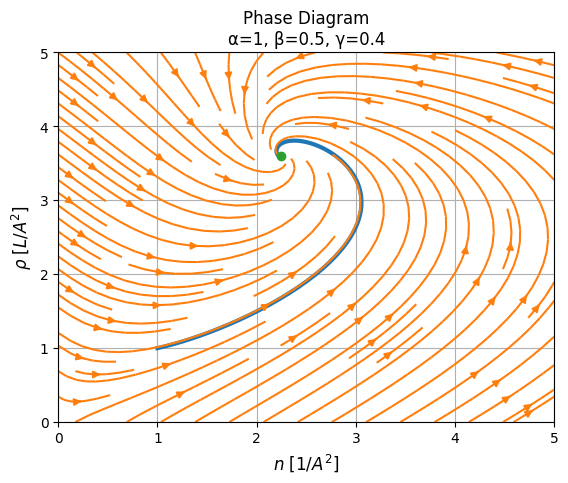
\includegraphics[width=0.5\linewidth]{images/simpleODEModel1PhasePortrait}

	\label{fig:simpleodemodel1phaseportrait}
\end{figure}


Furthermore, the following diagram shows the nullclines and the sign of the vector field at the different regions of the phase portrait.

\FloatBarrier

%\begin{strangeObs}
%	This equilibrium point $p^0_1$ has no choice but to be stable, if we expect the model to represent real biological situation. But our analysis above, reveals that this equilibrium point is in fact a saddle point. However, I can argue that if that the eigenvector with negative eigenvalue for the Jacobian matrix evaluated at $p^0_2$, lies in the first quadrant, then $p^0_2$ will ``look'' stable for the points at the first quadrant. But I am not sure if this is something normal to happen for a biological model.
%\end{strangeObs}


\subsection*{Quantitative analysis with nullclines}
Drawing the phase portrait and including the nullclines helps in understanding the quantitative effect of change in parameters (which causes by the drug-vessel interaction). To draw the nullclines, we require
\[ \vectt{\dot{n}}{\dot{\rho}} = \vectt{f_1(n,\rho)}{f_2(n,\rho)} = \vectt{\frac{\alpha}{\beta}n + \rho - n\rho}{\frac{\gamma}{\beta^2}n - \rho} = \vectt{0}{0}. \]
After a little bit of algebra, we get
\begin{align*}
	\dot{n} = 0:& \qquad \rho = \frac{\alpha}{\beta}\cdot \frac{n}{n-1} \quad (n\neq 1),\\
	\dot{\rho} = 0:& \qquad \rho = \frac{\gamma}{\beta^2}n.
\end{align*}
\begin{observation}
	The reason that we get the restriction $n\neq 1$ for the $\dot{n} = 0$ nullcline is the following. From (E.1.1) we know that $f_1(p^0_2)=0$. Thus we can use the implicit function theorem to get a continuous branch of equilibria near $p_2^0$ in the form of $\rho = \hat{\rho}(n)$ where $\hat{\rho}$ is a continuously differentiable function, where $\rho^* = \hat{\rho}(n^*)$ (note $p^0_2 = (n^*, \rho^*)$), and $f_1(n,\hat{\rho}(n)) = 0$ for some neighborhood of $p_0^2$. However, we can use this implicit function argument only when $\partial_\rho f_1 \neq 0$, which implies $n\neq 1$.\\
	Also, it is interesting to note that $n=1$ is equivalent to $\alpha=0$. This can be observed from (E.1.1). The consequences of this are summarized in the following observation boxes.
\end{observation}

We will have two cases of the phase portrait as shown in the figure below. Note that the stability of the equilibrium point $p_2^0$ will still remain the same as the value of $\alpha$ passes $\alpha=0$ transversally. The results of this section is summarized in the observation box below.
\begin{figure}[h!]
	\centering
	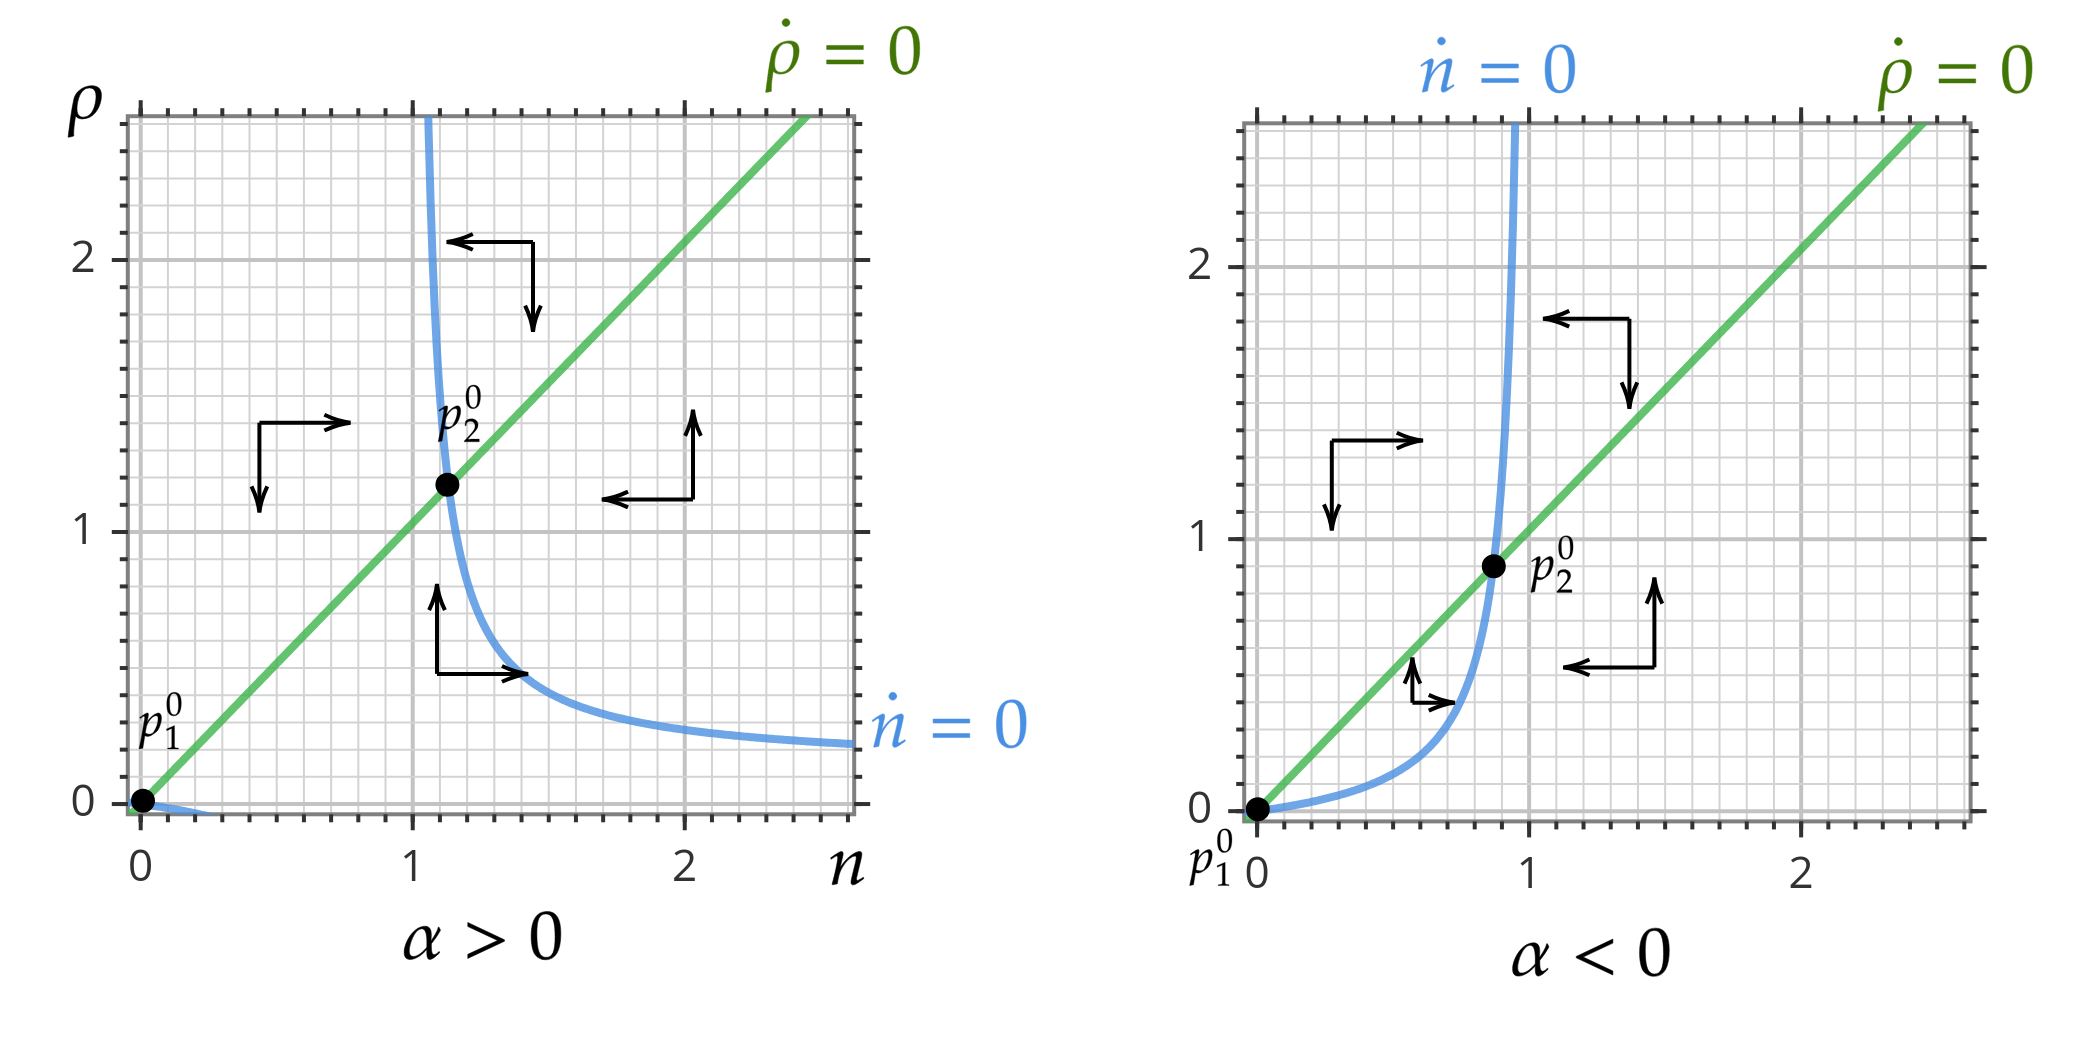
\includegraphics[width=\linewidth]{images/nullClines_positiveNegative.png} % first image
\end{figure}

\FloatBarrier

\begin{observation}[Two different phase portraits]
	As the parameter $\alpha$ passes through $\alpha_0 = 0$ transversally, we get two phase portraits that are not topologically equivalent (the results are shown in the figure above). Because of this, depending on the sign of $\alpha$, we will observe totally different behaviours from the system as we change the parameter values. \\
	I \textbf{emphasis} that in both of these phase portraits, the stability of both equilibria remains the same.
\end{observation}

\begin{observation}[Biological meaning of $\alpha$]
	From $(\clubsuit)$ we see that $\alpha = \lambda_s - \delta_t$, where $\lambda_s$ is the tip cell division rate (which leads to vascular splitting), and $\delta_t$ is the death rate of the tip cells. Thus $\alpha >0$ translates to larger division rate compared to the death rate for tip cells, and $\alpha<0$ is the opposite.
\end{observation}





\subsection*{Quantitative study of Effect of Changing the Parameters}
This section will lay the foundations for studying the drug-vessel interaction and how that affects the system.
\subsubsection*{Effect of $\alpha$} 
Regardless of the sign of $\alpha$ (i.e. being in either of phase portraits) increasing the value of alpha will move the $p^0_2$ higher. This observation is summarized in the following figure.
\begin{figure}[h!]
	\centering
	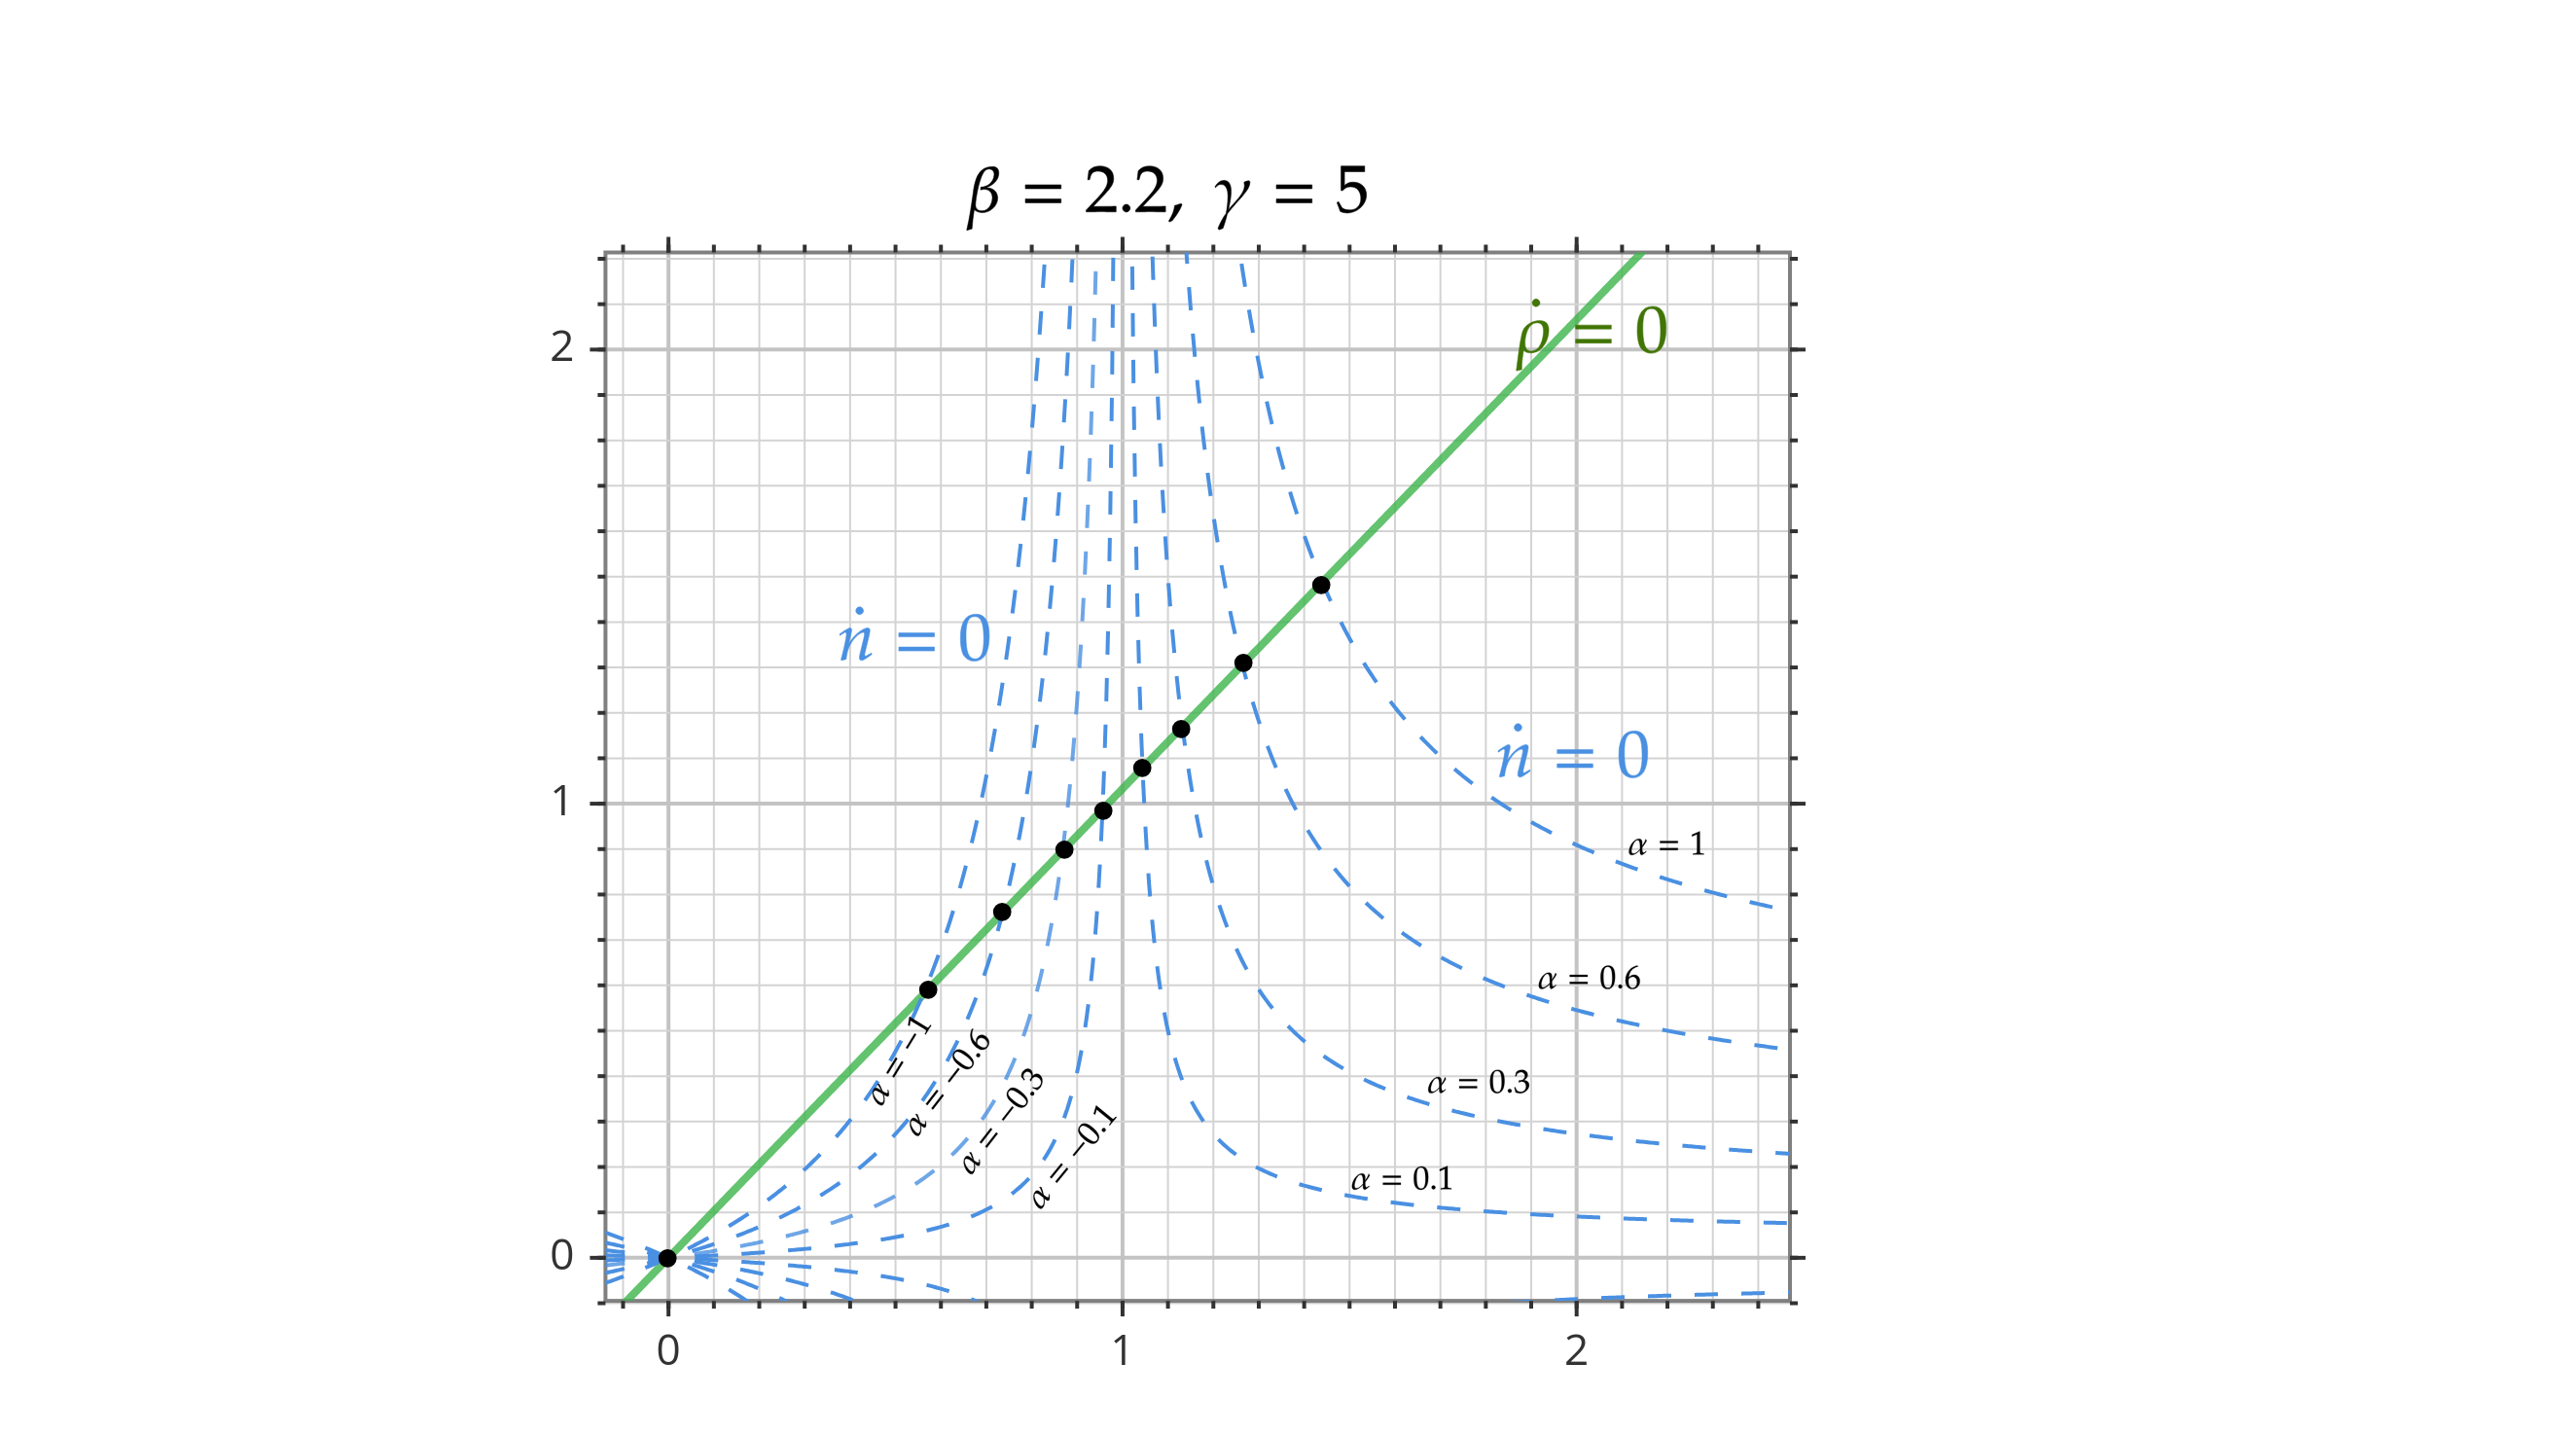
\includegraphics[width=\linewidth]{images/effectOfAlpha.png} % first image
\end{figure}

\FloatBarrier

\subsubsection*{Effect of $\gamma$}
$\gamma$ is basically determining the slope of the $\dot{\rho}=0$ nullcline. The higher the value of $\gamma$ the more steeper is the slop. Thus changing the values of $\gamma$, the equilibrium point $p^0_2$ will move up or down on the $\dot{n}=0$ nullcline. The sign of $\alpha$ determines the way $p^0_2$ changes. The following figure summarizes the results for the argument above.

\begin{figure}[h!]
	\centering
	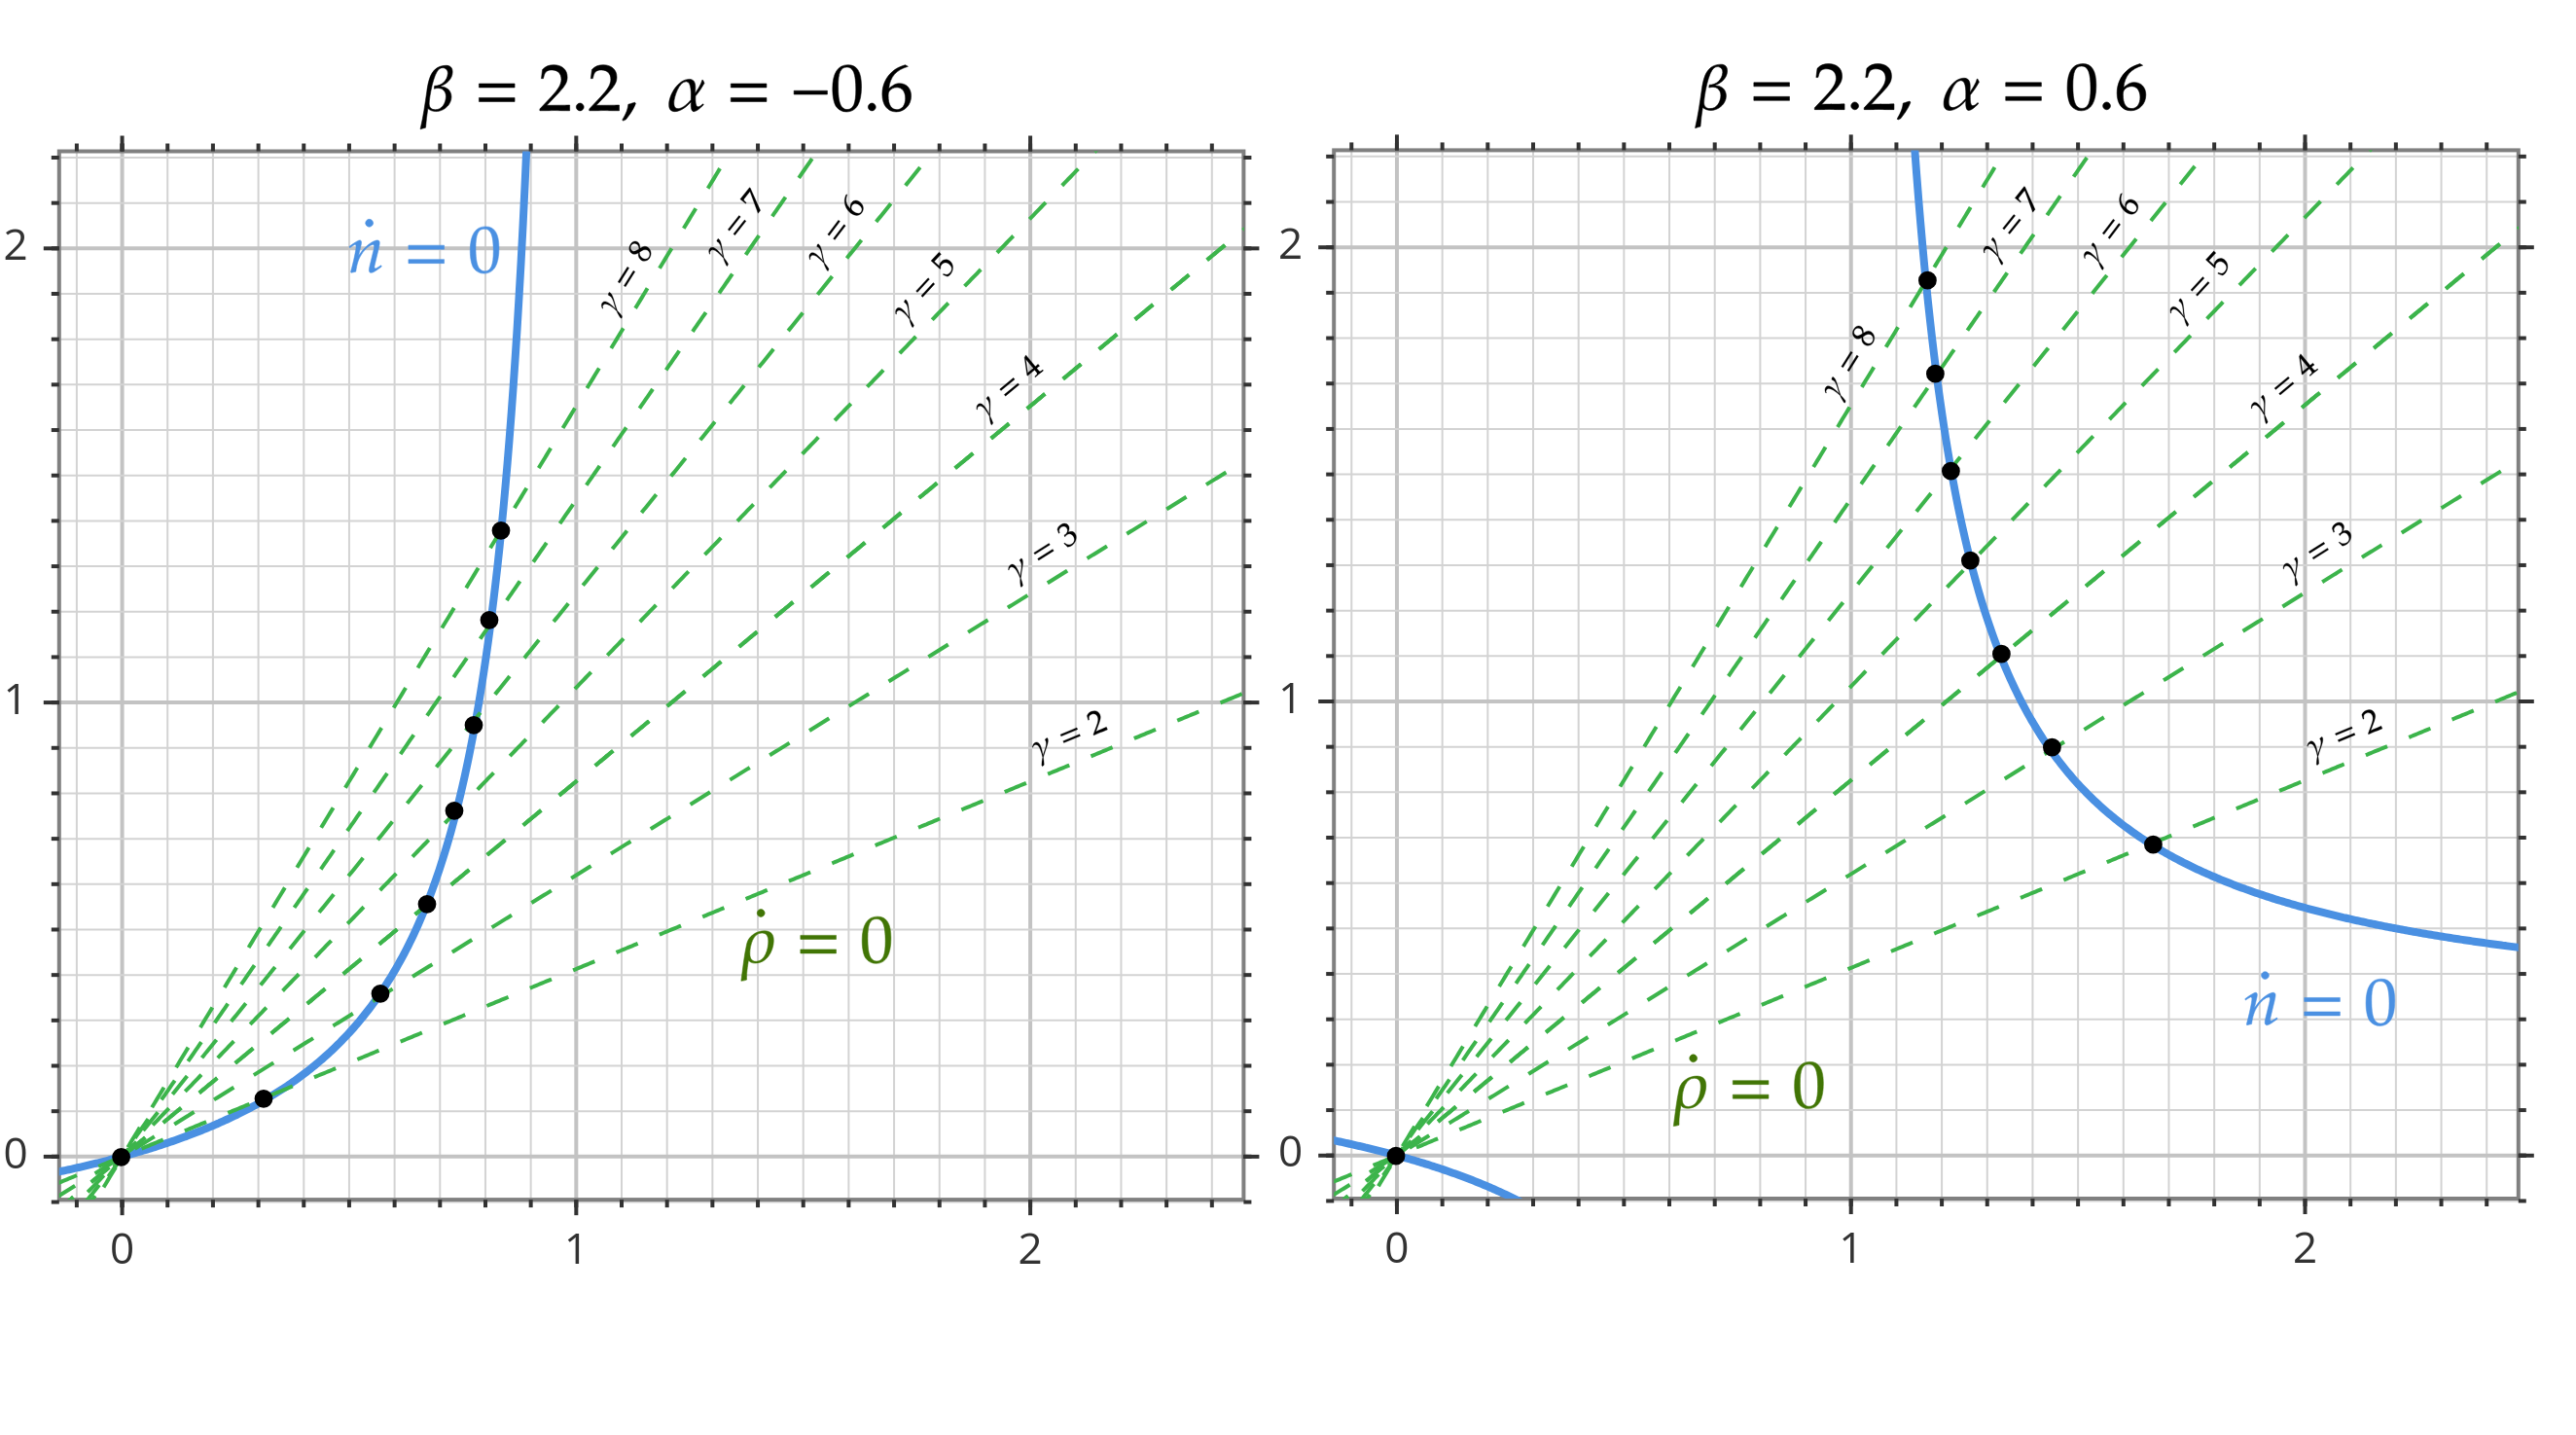
\includegraphics[width=\linewidth]{images/effectOfGamma.png} % first image
\end{figure}
\FloatBarrier

\subsubsection*{Effect of $\beta$}
Determining the effect of the parameter $\beta$ is not as straight forward as the other two parameters as it appears in both ODEs. However, we can plot the parameterized curve of $p^0_2(\beta)$ using (E.1.1) to see the effect of $\beta$ on the equilibrium point. The following figure summarizes the effect of $\beta$ on $p^0_2$.

\begin{figure}[h!]
	\centering
	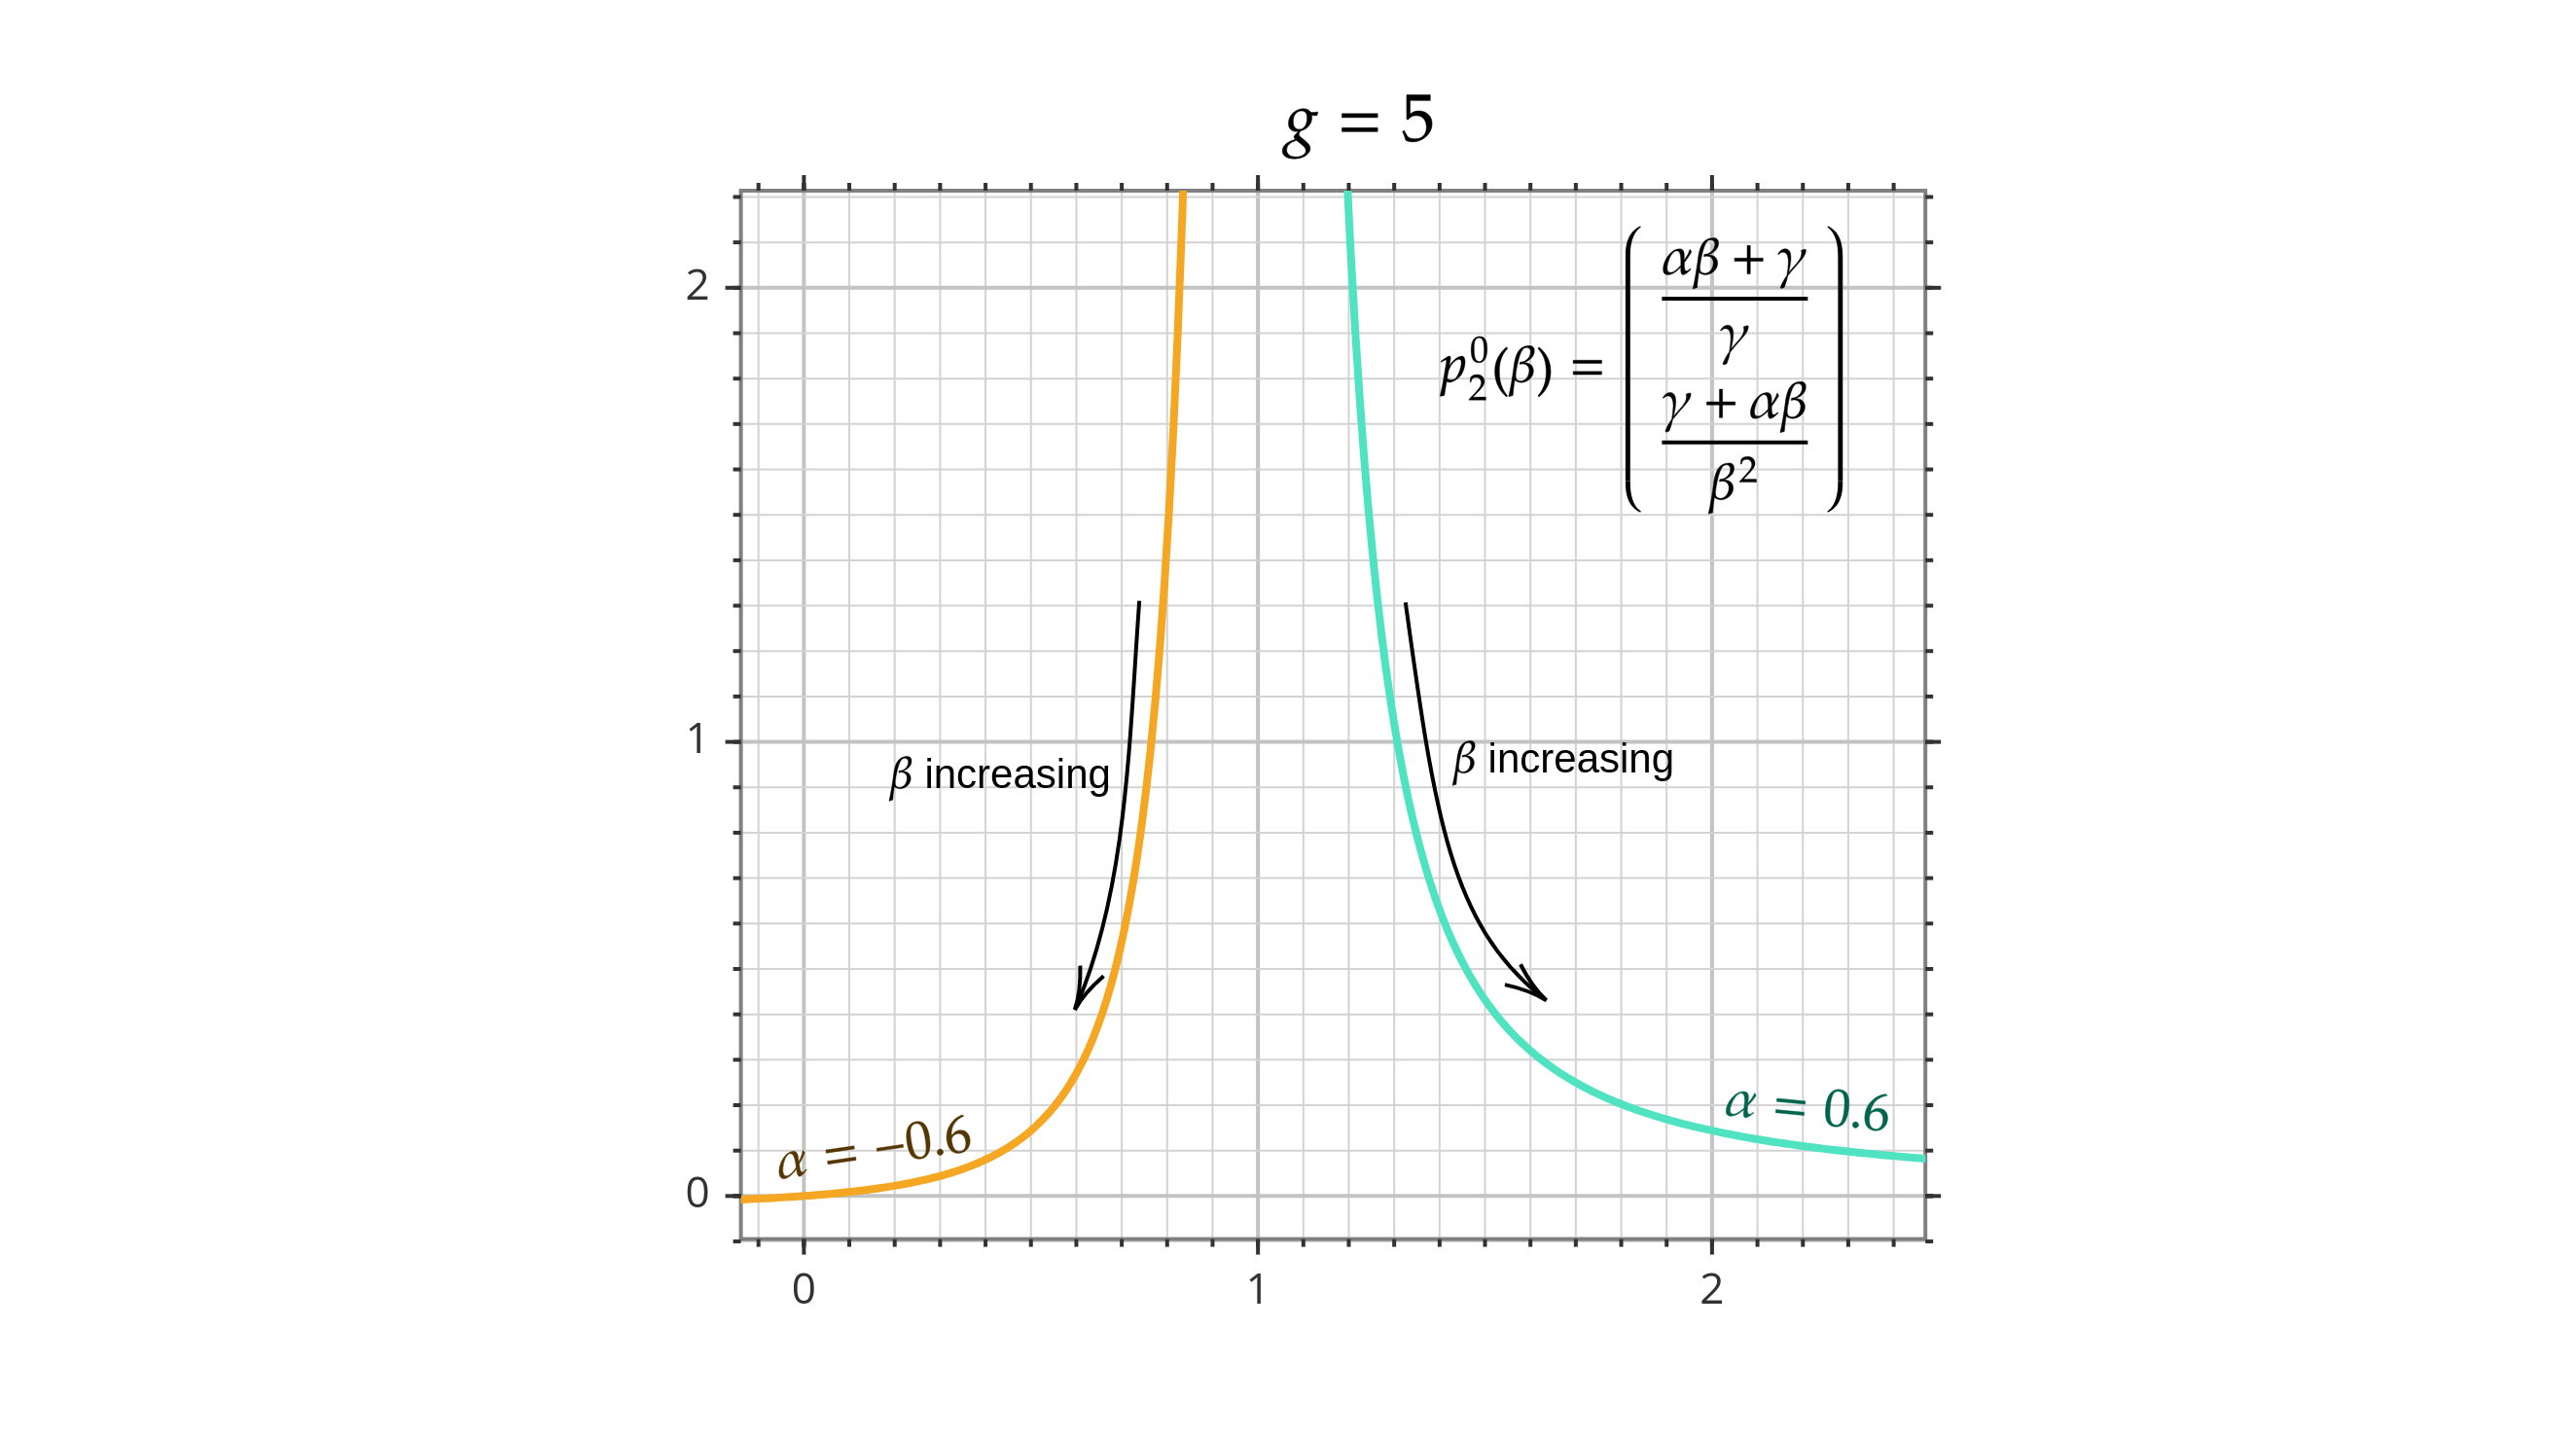
\includegraphics[width=\linewidth]{images/EffectOfBeta.png} % first image
\end{figure}
\FloatBarrier


\subsection*{Drug delivery}
In order to bring the drug-vessel interaction into play, we develop a ODE for $c(t)$ add approporite terms to the RHS of $\dot{n}$ and $\dot{\rho}$.
\[ \frac{dc}{dt} = \mu (\rho(t)f(t) - \sigma c(t)\rho(t)) - \boxed{\lambda c} \]
where $\mu$ has the unit [1/time], and $f(t)$ is the amount drug inside the capillary that has the unit [nmol per unit length]. Note that we have assumed the exchange of drug between the vessels and the region of interest is proportional to the difference in the concentration of drug in two different environments. Furthermore, the coefficient $\sigma$ has the units of [area/length] which is an indicator of the area coverage of the blood vessels. This parameter somehow characterizes the space filling and fractal structure of the blood vessels. This parameter should have some relations with the fractal dimension of a given vascular structure. Considering the dynamics of this parameter can possibly reflect some of the topological and non-local characterizations of the vascular network.



\subsubsection*{Basic and Simplified delivery scenario}
We assume that there is an infinite pool of drug (i.e. the patient is getting injected continuously) so the amount of drug per unit length in the capillary is constant $C_0$ [nmol per unit length].
\[ \frac{dc}{dt} = \mu \rho(t)(C_0 - \sigma c(t)).  \]

Also, note that we have ignored the radiation decay term to keep stuff simpler at this stage. The reason behind this choice is that at this stage, in adding the drug-vessel interaction, we will only consider a mass-action type interaction (i.e. chemical interactions), and no radio-biological interaction will be assumed (which has more complexity).

Another assumption that we make is that since the molecules of the drug are much smaller and simpler than the cells in the body, then we assume that they reach to equilibrium much more faster than the characteristic time scale of tip cell movement, and the death/generation of the cells. This basically means that we can simply assume $dc/dt=0$ to arrive at the following algebraic equation for $c$.
\[ C_0 = \sigma c(t). \]



\subsection*{Adding the drug-vessel interaction}
Presence of drug in the environment can have many different effects. It can kill/deactivate the existing tip cells (increasing $\delta_t$). Or it can change the rate at which the endothelial cells turn into the tip cells (changing the value of $\delta_b$). Or it can affect the tip cell division rate ($\lambda_s$). It can also affect the cellular migration of the tip cells and change the value of parameter $v$. The following lists the parameters corresponding to the amplitude of each of these interactions
\begin{itemize}
	\item $a_1$: changing the tip cell movement/migration
	\item $a_2$: killing/deactivating the tip cells
	\item $a_3$: changing the endothelial-to-tip cell conversion rate
	\item $a_4$: changing the tip cell division rate
\end{itemize}


\subsection*{Some discussions on drug interaction}
In mathematical modeling of biological processes, incorporating drug interactions can be complex, as the drug can influence various parameters of the system in different ways. The choice of interaction term often depends on the nature of the drug action and the available experimental data.
Here are a few common approaches to include drug interactions in the model:

\begin{enumerate}
	\item \textbf{Linear Interaction}: If the drug effect is proportional to its concentration, we can model the interaction linearly. For instance:
	\begin{align*}
		v(c) &= v_0 - a_1 c, \\
		\delta_v(c) &= \delta_{v0} + a_2 c,\\
		\lambda_b(c) &= \lambda_{b0} + a_3 c,\\
		\lambda_s(c) &= \lambda_{s0} - a_4 c.
	\end{align*}
	Here, \( v_0 \) and \( \delta_{v0} \) are the baseline motility and degradation rates without the drug, while \( a_1 \) and \( a_2 \) represent the sensitivity of these rates to the drug concentration. Similarly \( \lambda_{b0} \) and \( \lambda_{s0} \) are the baseline rates without the drug, and \( a_3 \), \( a_4 \) are the sensitivities of these rates to the drug concentration.

	
	\item \textbf{Hill Function}: If the drug effect exhibits saturation -- meaning it has a maximum effect regardless of concentration -- a Hill function can be appropriate:
	\begin{align*}
		v(c) &= v_0 \left(1 - \frac{a_1 c^h}{K_d^h + c^h}\right), \\
		\delta_v(c) &= \delta_{v0} \left(1 + \frac{a_2 c^h}{K_d^h + c^h}\right),\\
		\lambda_b(c) &= \lambda_{b0} \left(1 + \frac{a_3 c^h}{K_{d3}^h + c^h}\right),\\
		\lambda_s(c)& = \lambda_{s0} \left(1 - \frac{a_4 c^h}{K_{d4}^h + c^h}\right),
	\end{align*}
	Here, \( h \) is the Hill coefficient that determines the steepness of the response curve, and \( K_d \) is the drug concentration at which the effect is half of its maximum. With \( h \) as the Hill coefficient, and \( K_{d3} \), \( K_{d4} \) as the half-maximal effective concentrations for \( \lambda_b \) and \( \lambda_s \), respectively.
	
	\item \textbf{Michaelis-Menten Kinetics}: If the drug interaction is enzyme-like, you can model it using Michaelis-Menten kinetics:
	\begin{align*}
		v(c) &= v_0 \left(1 - \frac{a_1 c}{K_m + c}\right), \\
		\delta_v(c) &= \delta_{v0} \left(1 + \frac{a_2 c}{K_m + c}\right),\\
		\lambda_b(c) &= \lambda_{b0} \left(1 + \frac{a_3 c}{K_m + c}\right),\\	
		\lambda_s(c) &= \lambda_{s0} \left(1 - \frac{a_4 c}{K_m + c}\right),
	\end{align*}
	Where \( K_m \) is the Michaelis constant, representing the drug concentration at which the rate of reaction is half of its maximum. where \( K_m \) is the Michaelis constant, indicative of the concentration at which the reaction rate is half its maximum.
	
	\item \textbf{Exponential or Sigmoidal Functions}: For more complex drug effects, such as those that have a threshold effect or exhibit a sigmoidal dose-response, exponential or sigmoidal functions can be used.
\end{enumerate}

These interaction terms would be incorporated into the model by modifying the differential equations as follows:
\[
\frac{d\rho}{dt} = v(c)n - \delta_v(c) \rho,
\]

\[
\frac{dn}{dt} = (\lambda_s(c) - \delta_t) n + \lambda_b(c) \rho - \kappa n \rho,
\]

where \( \lambda_b(c) \) and \( \lambda_s(c) \) are now functions of the drug concentration that reflect the modulation of the endothelial-to-tip cell conversion rate and the tip cell division rate by the drug.

The form of the interaction should be chosen based on the biological mechanism of the drug action, the type and quality of experimental data available, and the ability to estimate the additional parameters introduced by these functional forms with the available data.
To decide which model to use, consider the following:

\begin{itemize}
	\item \textbf{Biological Mechanism}: Does the drug interact with its target in a manner that is competitive, non-competitive, or does it follow some form of cooperative binding? This will guide whether you use linear, Hill, or Michaelis-Menten kinetics.
	\item \textbf{Data Availability}: What kind of data do you have? If you have dose-response data, you can fit these models to the data to estimate parameters like \( a_1 \), \( a_2 \), \( h \), \( K_d \), or \( K_m \).
	\item \textbf{Parameter Estimation}: Can you estimate the additional parameters introduced by these functions? More complex models require more data for accurate parameter estimation.
\end{itemize}





\newpage

\section{Some Ideas to Try}
This section might have very simple, basic and sometimes silly ideas that came into my mind during developing some models and I thought they might worth trying
\begin{itemize}
	\item Developing a model for a weighted graph generation. I suspect a weighted graph might have all the necessary information we want.
\end{itemize}